\let\RaggedRight\raggedright
\let\raggedright\relax
\documentclass[utf8,9pt,mathserif,usepdftitle=false]{beamer}

\usepackage{graphicx}%
\usepackage{float}%
\usepackage{wrapfig}%

\let\RaggedRight\raggedright
\let\raggedright\relax
\documentclass[utf8,9pt,mathserif,usepdftitle=false]{beamer}

\usepackage{graphicx}%
\usepackage{float}%
\usepackage{wrapfig}%

\let\RaggedRight\raggedright
\let\raggedright\relax
\documentclass[utf8,9pt,mathserif,usepdftitle=false]{beamer}

\usepackage{graphicx}%
\usepackage{float}%
\usepackage{wrapfig}%

\let\RaggedRight\raggedright
\let\raggedright\relax
\documentclass[utf8,9pt,mathserif,usepdftitle=false]{beamer}

\usepackage{graphicx}%
\usepackage{float}%
\usepackage{wrapfig}%

\include{present.daf}

% \setbeameroption{show notes on second screen}
\setbeameroption{hide notes}
\mode<presentation>
{
  \usetheme{default}
  %\usecolortheme{default} % dove, beaver
  \usecolortheme{whale}
  %\usefonttheme{serif}
}

\hypersetup{%
  pdfinfo={%
    Title={Защита курсовых работ, ИГУ},%
    Subject={О воспроизводимости результатов численных решений уравнения осцилляции нейтрино в среде},%
    Author={Данеко Илья},%
    Keywords={neutrino oscillation in matter;quality properties}%
  }
}

\title{Качественные свойства решений уравнения осцилляций нейтрино в среде
}%
\author{Данеко И.И.}
\date[ИГУ, 2025]{%
  20 октября 2025\\%
  \vspace*{10ex}%
  \begin{flushright}
    \small
    Научный руководитель: Ломов В.П.\par
  \end{flushright}
  {\vspace*{7ex}
    \footnotesize%
    Иркутск, ФГБОУ ВО ИГУ\par%
  } }

\begin{document}

\begin{frame}
  \titlepage
\end{frame}

\begin{frame}
  \frametitle{Введение}%
  %%%
  % TODO:
  \begin{itemize}
  \item<1->
   Нейтрино — одна из самых необычных частиц в нашем мире.
   
   \item<2->
   Она обладает нулевым зарядом, полуцелым спином и участвует только в слабом
   взаимодействии.
  
  \item<3-> 
  Нейтрино существует как бы в двух видах: флейворные нейтрино и
  массивные. Первые рождаются, тогда как вторые — распространяются.
 
  
  \item<4->% 
   В данной работе мы разбираем качественные
  характеристики численного решения уравнения осцилляции нейтрино в среде.
  \end{itemize}
\end{frame}

\begin{frame}
  \frametitle{Осцилляции нейтрино}%
  %%%
  Три известных состояния флейворных  \({\nu_{\alpha}}(\alpha= e, \mu, \tau)\) являются линейными комбинациями состояний массивных \({\nu_{i}}\) c массами \(m_{i}(i=1,2,3)\), состояния флейворных нейтрино являются суперпозицией состояний массивные нейтрино
  
  \onslide<2->%
  \begin{equation*}\label{eq:1}
  	{\nu_{\alpha}}=\sum_{i}U_{\alpha i}^{*}{\nu_{i}},
  \end{equation*} 
  \(U_{\alpha i}\) являются элементами унитарной матрицы
  смешивания и называемой матрицей Понтекорва–Маки–Накагавы–Сакаты (PMNS).
  
  \onslide<3->%
  Вероятность иметь состояние аромата \(\beta\) в точке r
  \begin{equation*}
  	P_{\alpha\beta}=\sum_{j}|U_{\beta j}|^{2}|A_{j}|^{2}+2\sum_{i>j}Re[U_{\beta i}U_{\beta j}^{*}A_{i}A_{j}^{*}\exp^{-\imath\Delta_{ij}L}].
  \end{equation*}
  Здесь \(\Delta_{ij}=\Delta m_{ij}^2/2E\), где \(E=|p|\), а \(A_{i}\) амплитуда вероятности наличия в точке регестрации
\end{frame}

\begin{frame}
  \frametitle{Осцилляции нейтрино в веществе}%
  %%%
  Уравнение осцилляций в среде
  \begin{equation*}
  	\imath \frac{\partial \Psi}{\partial \xi}=H(\xi)\Psi(\xi).\quad
  \end{equation*}
   \onslide<2->%
  Здесь \({H(\xi)}\) — эрмиртовая матрица
  \begin{equation*}
  	H(\xi)=H_0+\upsilon(\xi)W
  \end{equation*}
   \onslide<3->%
  Матрица \(W\) имеет вид:
  \begin{equation*}
  	W=
  	\begin{pmatrix}
  		c_{13}^{2}c_{12}^{2} & c_{12}s_{12}c_{13}^{2} & c_{12}c_{13}s_{13}\\
  		c_{12}s_{12}c_{13}^{2} & s_{12}^{2}c_{13}^{2} & s_{12}c_{13}s_{13}\\
  		c_{12}s_{13}c_{13} & s_{12}c_{13}s_{13} & s_{13}^{2}
  	\end{pmatrix}.
  \end{equation*}

  \onslide<4->%
  Профиль плотности для солнечной модели
  
  \begin{equation*}
  	\upsilon(\xi)=\gamma exp(-\eta\xi)
  \end{equation*}
  

\end{frame}

\begin{frame}
  \frametitle{Наблюдаемые}%
  %%%
  Вероятность иметь состояние аромата \(\beta\) в точке r
  \begin{equation*}
  	P_{\alpha\beta}=\sum_{j}|U_{\beta j}|^{2}|A_{j}|^{2}+2\sum_{i>j}Re[U_{\beta i}U_{\beta j}^{*}A_{i}A_{j}^{*}\exp(-\imath\Delta_{ij}L)].
  \end{equation*}
  
  \onslide<2->%
  средняя вероятность выживания составляет
  \begin{equation}
  	\langle P_{ee} \rangle=c_{12}^{2}c_{13}^{2}|\Psi_{1}|^{2}+s_{12}^{2}c_{13}^{2}|\Psi_{2}|^{2}+s_{13}^{2}|\Psi_{3}|^{2}.
  \end{equation}
\end{frame}

\begin{frame}
	\frametitle{Качественные свойства решения}%
	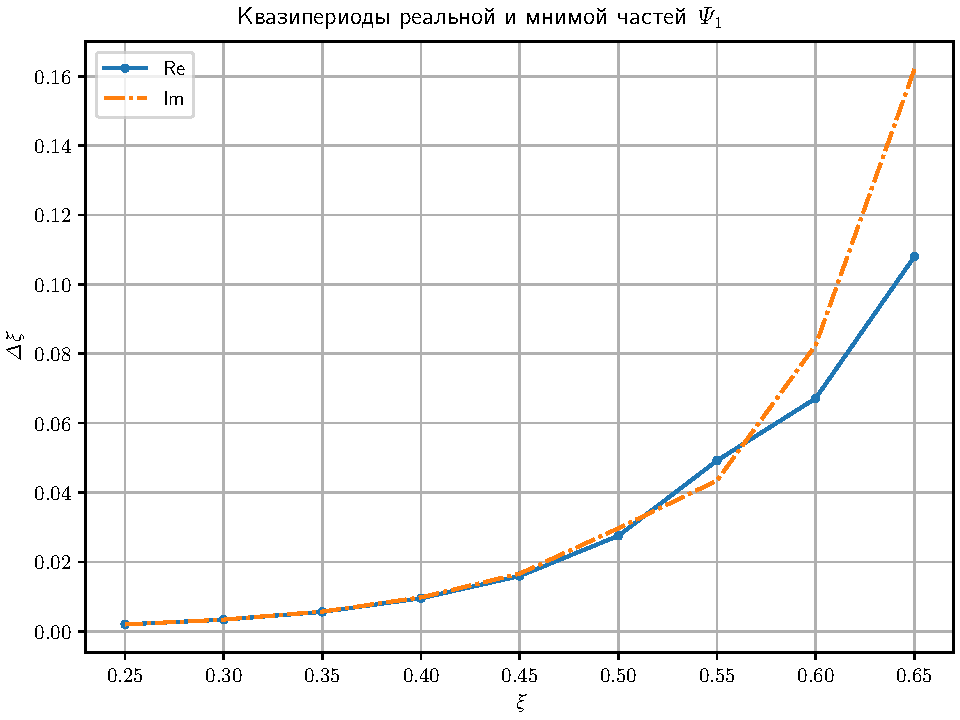
\includegraphics[width=\linewidth]{ri-widths-ru}
\end{frame}

\begin{frame}
	\frametitle{Качественные свойства решения}%
	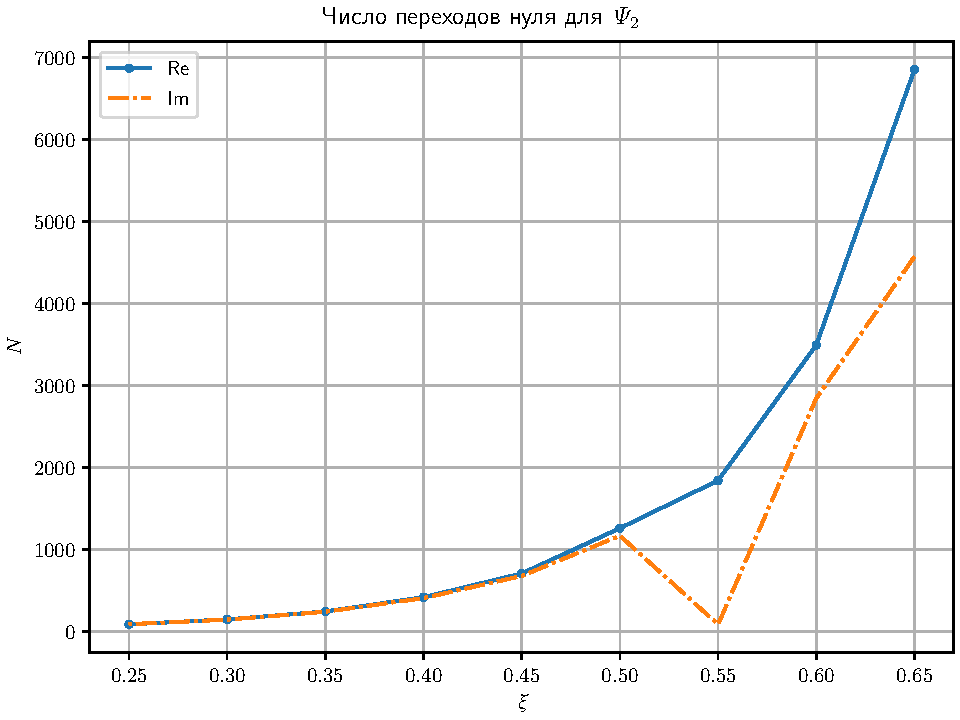
\includegraphics[width=\linewidth]{psi2-trans-ru}
\end{frame}

\begin{frame}
	\frametitle{Качественные свойства решения}%
	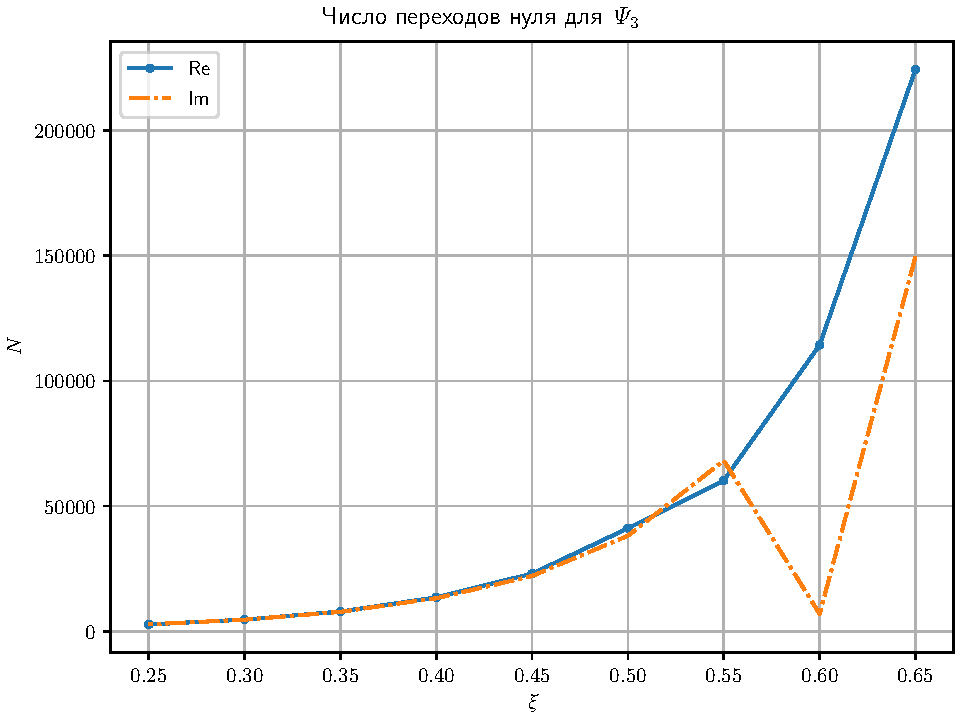
\includegraphics[width=\linewidth]{psi3-trans-ru}
\end{frame}

\begin{frame}
	\frametitle{Качественные свойства решения}%
	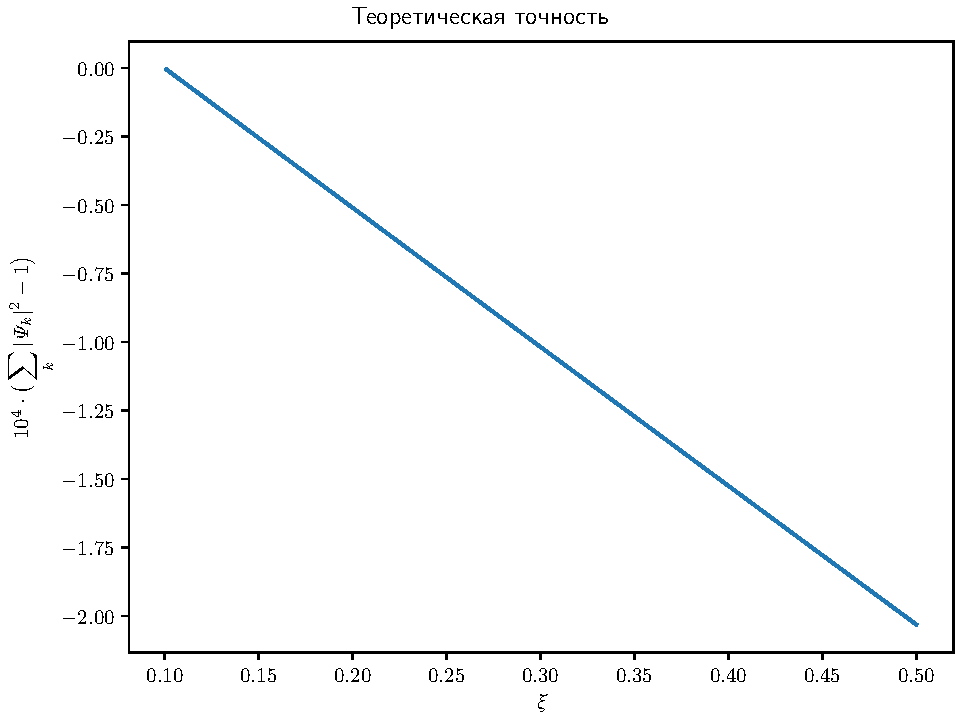
\includegraphics[width=\linewidth]{control-scaled}
\end{frame}

\begin{frame}
	\frametitle{Качественные свойства решения}%
	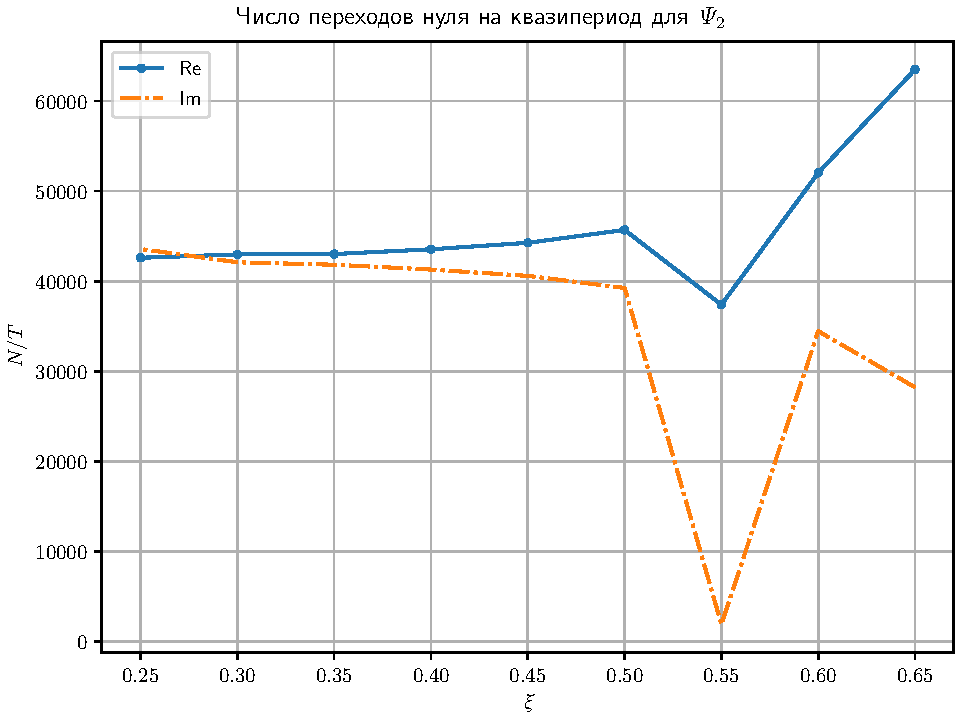
\includegraphics[width=\linewidth]{psi2-rel-trans-ru}
\end{frame}

\begin{frame}
	\frametitle{Качественные свойства решения}%
	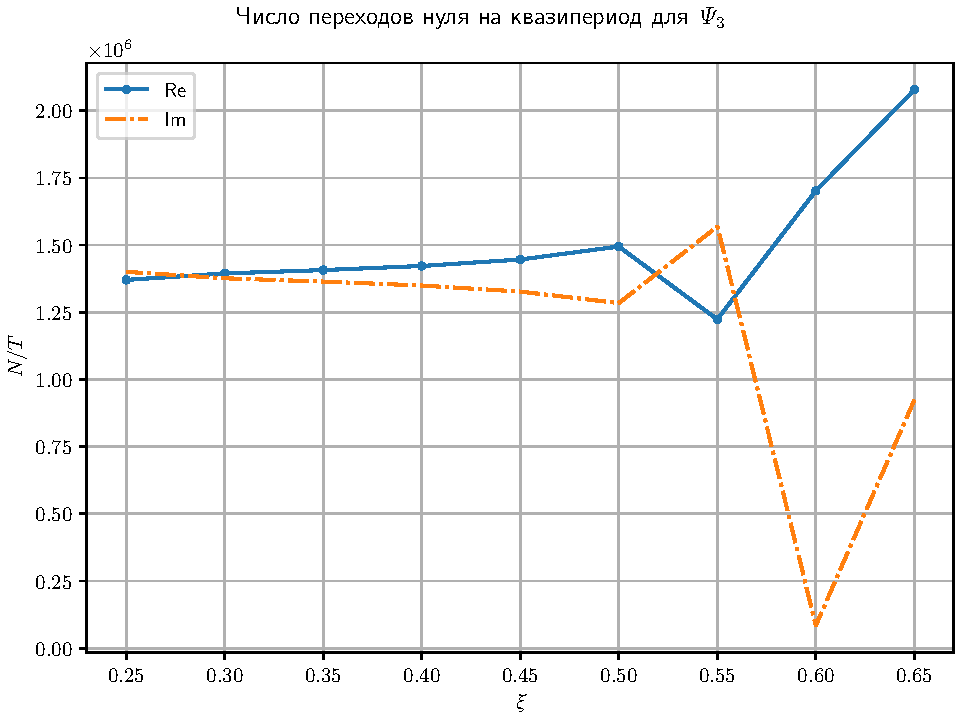
\includegraphics[width=\linewidth]{psi3-rel-trans-ru}
\end{frame}

\begin{frame}
  \frametitle{Заключение}%
  %%%
  В данной работе мы применили встроенные в Mathematica средства численного
  решения дифференциальных уравнений (DOPRI) для выясления качественных
  характеристик полученного решения. 
  \begin{itemize}
  \onslide<2->%
  \item<1-> Мы нашли подходящую характеристику.
  \onslide<3->%
  \item<2->следует внимательно относиться к расчётам с помощью встроенных средств и, по возможности, использовать альтернативные алгоритмы.
  \end{itemize}
\end{frame}

\begin{frame}
  \frametitle{КОНЕЦ}%
  \LARGE%
  \centering%
  \bfseries%
  СПАСИБО ЗА ВНИМАНИЕ%
\end{frame}

\begin{frame}
  \frametitle{Дополнительно}%
  %%%
  \centering%
  ДОПОЛНИТЕЛЬНЫЙ МАТЕРИАЛ
\end{frame}

\end{document}

%%% Local Variables:
%%% mode: latex
%%% fill-column: 80
%%% TeX-master: t
%%% TeX-PDF-mode: t
%%% End:
%%% vim: syn=tex ft=tex tw=80 ts=2 sw=2 et:


% \setbeameroption{show notes on second screen}
\setbeameroption{hide notes}
\mode<presentation>
{
  \usetheme{default}
  %\usecolortheme{default} % dove, beaver
  \usecolortheme{whale}
  %\usefonttheme{serif}
}

\hypersetup{%
  pdfinfo={%
    Title={Защита курсовых работ, ИГУ},%
    Subject={О воспроизводимости результатов численных решений уравнения осцилляции нейтрино в среде},%
    Author={Данеко Илья},%
    Keywords={neutrino oscillation in matter;quality properties}%
  }
}

\title{Качественные свойства решений уравнения осцилляций нейтрино в среде
}%
\author{Данеко И.И.}
\date[ИГУ, 2025]{%
  20 октября 2025\\%
  \vspace*{10ex}%
  \begin{flushright}
    \small
    Научный руководитель: Ломов В.П.\par
  \end{flushright}
  {\vspace*{7ex}
    \footnotesize%
    Иркутск, ФГБОУ ВО ИГУ\par%
  } }

\begin{document}

\begin{frame}
  \titlepage
\end{frame}

\begin{frame}
  \frametitle{Введение}%
  %%%
  % TODO:
  \begin{itemize}
  \item<1->
   Нейтрино — одна из самых необычных частиц в нашем мире.
   
   \item<2->
   Она обладает нулевым зарядом, полуцелым спином и участвует только в слабом
   взаимодействии.
  
  \item<3-> 
  Нейтрино существует как бы в двух видах: флейворные нейтрино и
  массивные. Первые рождаются, тогда как вторые — распространяются.
 
  
  \item<4->% 
   В данной работе мы разбираем качественные
  характеристики численного решения уравнения осцилляции нейтрино в среде.
  \end{itemize}
\end{frame}

\begin{frame}
  \frametitle{Осцилляции нейтрино}%
  %%%
  Три известных состояния флейворных  \({\nu_{\alpha}}(\alpha= e, \mu, \tau)\) являются линейными комбинациями состояний массивных \({\nu_{i}}\) c массами \(m_{i}(i=1,2,3)\), состояния флейворных нейтрино являются суперпозицией состояний массивные нейтрино
  
  \onslide<2->%
  \begin{equation*}\label{eq:1}
  	{\nu_{\alpha}}=\sum_{i}U_{\alpha i}^{*}{\nu_{i}},
  \end{equation*} 
  \(U_{\alpha i}\) являются элементами унитарной матрицы
  смешивания и называемой матрицей Понтекорва–Маки–Накагавы–Сакаты (PMNS).
  
  \onslide<3->%
  Вероятность иметь состояние аромата \(\beta\) в точке r
  \begin{equation*}
  	P_{\alpha\beta}=\sum_{j}|U_{\beta j}|^{2}|A_{j}|^{2}+2\sum_{i>j}Re[U_{\beta i}U_{\beta j}^{*}A_{i}A_{j}^{*}\exp^{-\imath\Delta_{ij}L}].
  \end{equation*}
  Здесь \(\Delta_{ij}=\Delta m_{ij}^2/2E\), где \(E=|p|\), а \(A_{i}\) амплитуда вероятности наличия в точке регестрации
\end{frame}

\begin{frame}
  \frametitle{Осцилляции нейтрино в веществе}%
  %%%
  Уравнение осцилляций в среде
  \begin{equation*}
  	\imath \frac{\partial \Psi}{\partial \xi}=H(\xi)\Psi(\xi).\quad
  \end{equation*}
   \onslide<2->%
  Здесь \({H(\xi)}\) — эрмиртовая матрица
  \begin{equation*}
  	H(\xi)=H_0+\upsilon(\xi)W
  \end{equation*}
   \onslide<3->%
  Матрица \(W\) имеет вид:
  \begin{equation*}
  	W=
  	\begin{pmatrix}
  		c_{13}^{2}c_{12}^{2} & c_{12}s_{12}c_{13}^{2} & c_{12}c_{13}s_{13}\\
  		c_{12}s_{12}c_{13}^{2} & s_{12}^{2}c_{13}^{2} & s_{12}c_{13}s_{13}\\
  		c_{12}s_{13}c_{13} & s_{12}c_{13}s_{13} & s_{13}^{2}
  	\end{pmatrix}.
  \end{equation*}

  \onslide<4->%
  Профиль плотности для солнечной модели
  
  \begin{equation*}
  	\upsilon(\xi)=\gamma exp(-\eta\xi)
  \end{equation*}
  

\end{frame}

\begin{frame}
  \frametitle{Наблюдаемые}%
  %%%
  Вероятность иметь состояние аромата \(\beta\) в точке r
  \begin{equation*}
  	P_{\alpha\beta}=\sum_{j}|U_{\beta j}|^{2}|A_{j}|^{2}+2\sum_{i>j}Re[U_{\beta i}U_{\beta j}^{*}A_{i}A_{j}^{*}\exp(-\imath\Delta_{ij}L)].
  \end{equation*}
  
  \onslide<2->%
  средняя вероятность выживания составляет
  \begin{equation}
  	\langle P_{ee} \rangle=c_{12}^{2}c_{13}^{2}|\Psi_{1}|^{2}+s_{12}^{2}c_{13}^{2}|\Psi_{2}|^{2}+s_{13}^{2}|\Psi_{3}|^{2}.
  \end{equation}
\end{frame}

\begin{frame}
	\frametitle{Качественные свойства решения}%
	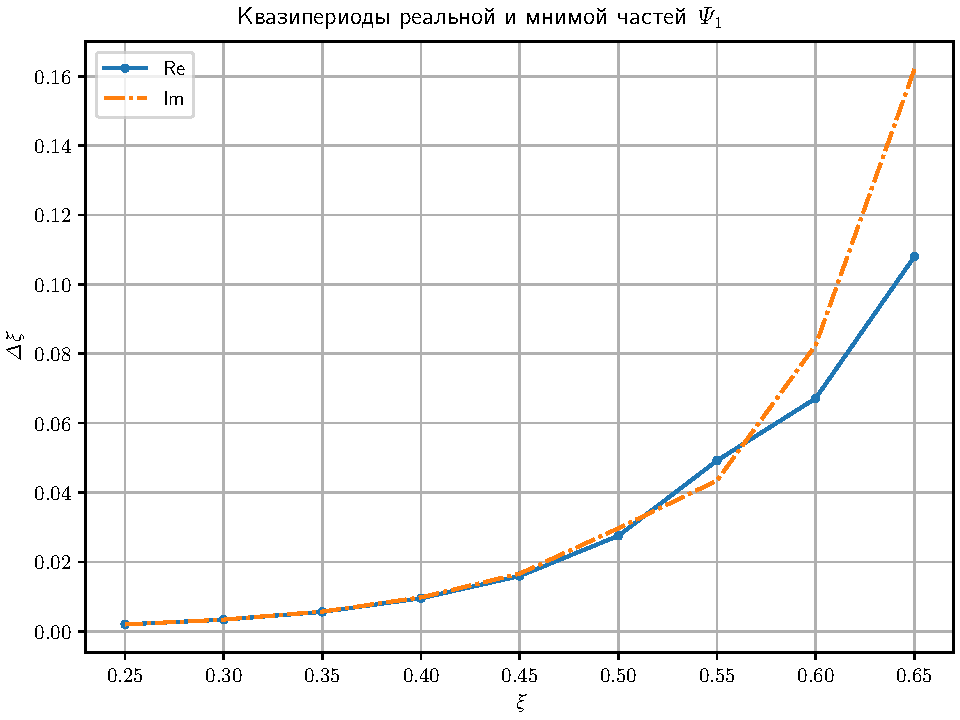
\includegraphics[width=\linewidth]{ri-widths-ru}
\end{frame}

\begin{frame}
	\frametitle{Качественные свойства решения}%
	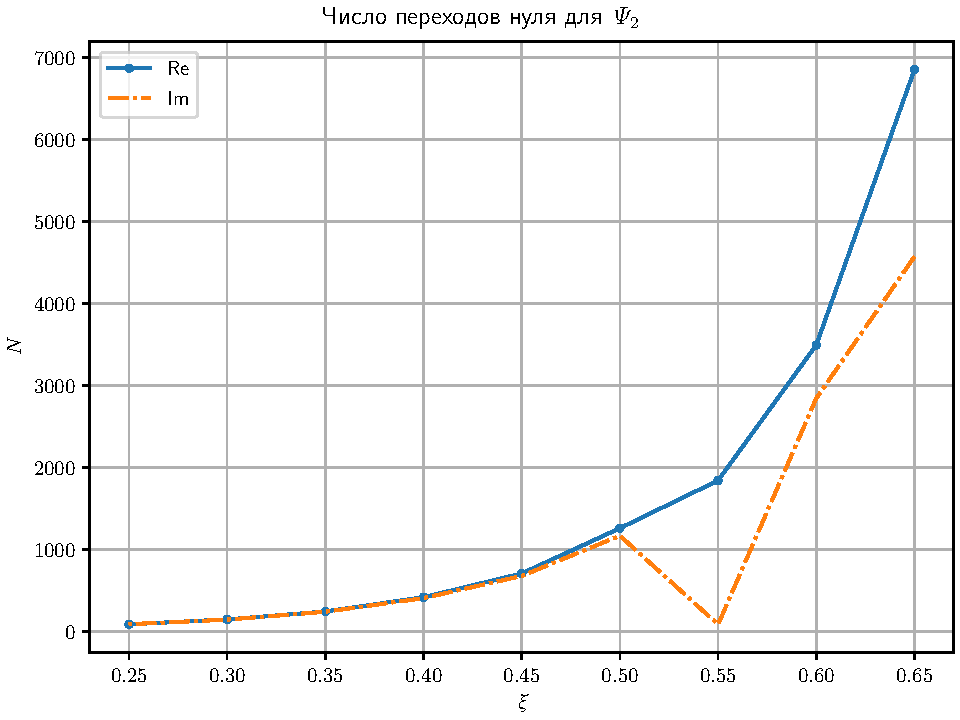
\includegraphics[width=\linewidth]{psi2-trans-ru}
\end{frame}

\begin{frame}
	\frametitle{Качественные свойства решения}%
	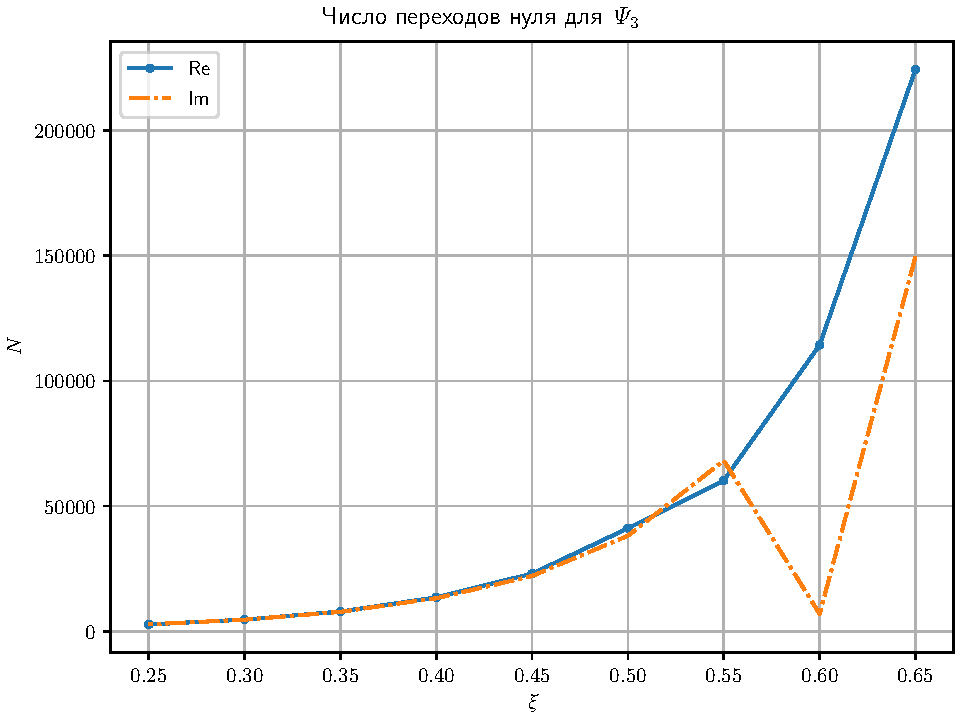
\includegraphics[width=\linewidth]{psi3-trans-ru}
\end{frame}

\begin{frame}
	\frametitle{Качественные свойства решения}%
	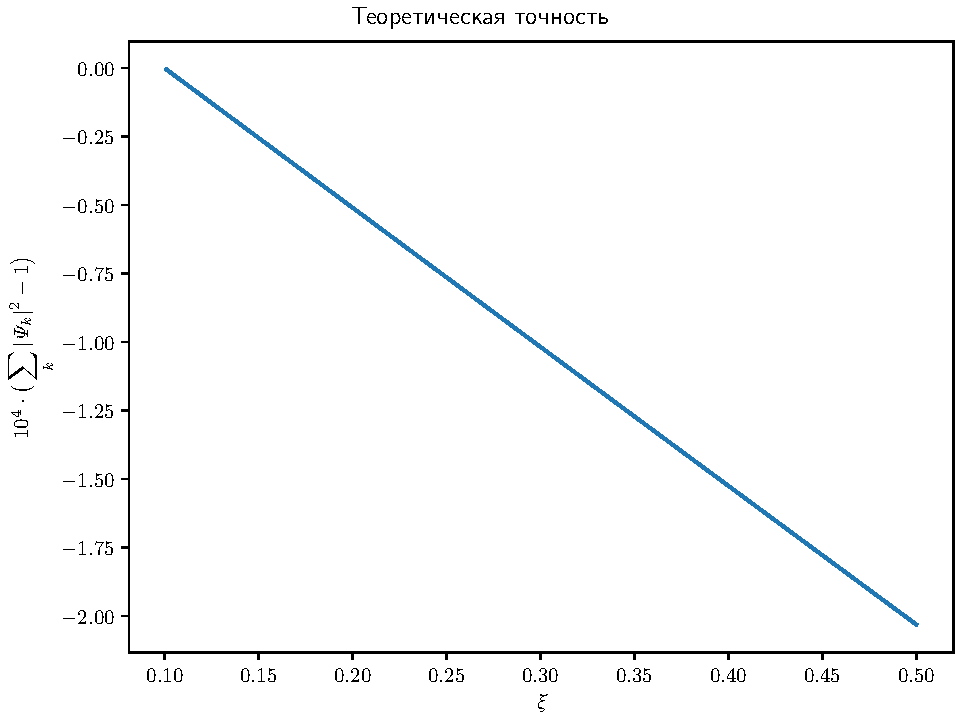
\includegraphics[width=\linewidth]{control-scaled}
\end{frame}

\begin{frame}
	\frametitle{Качественные свойства решения}%
	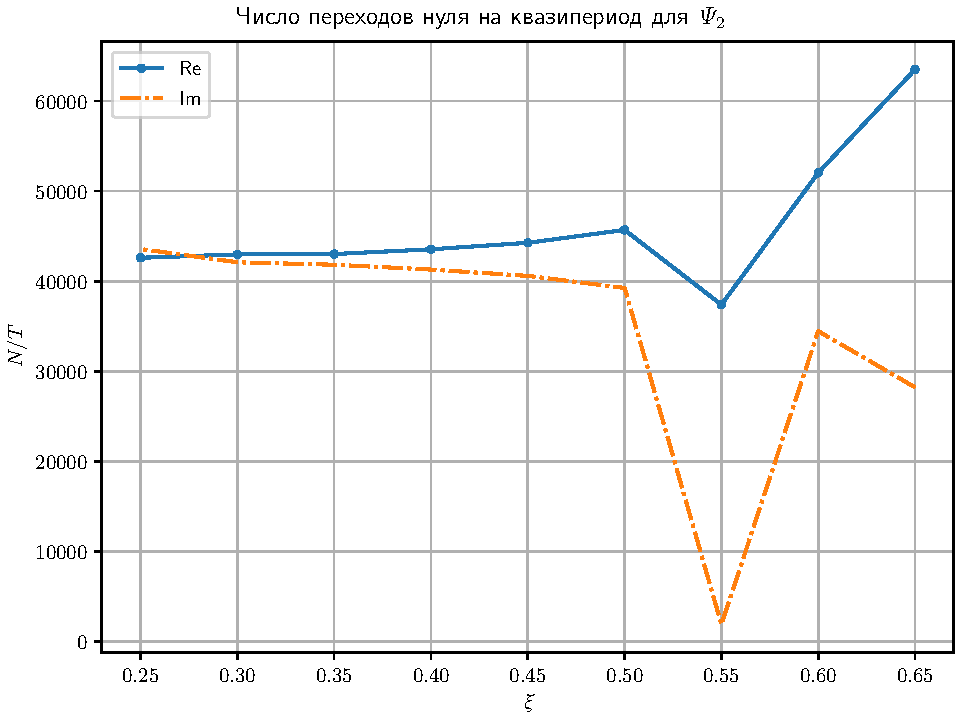
\includegraphics[width=\linewidth]{psi2-rel-trans-ru}
\end{frame}

\begin{frame}
	\frametitle{Качественные свойства решения}%
	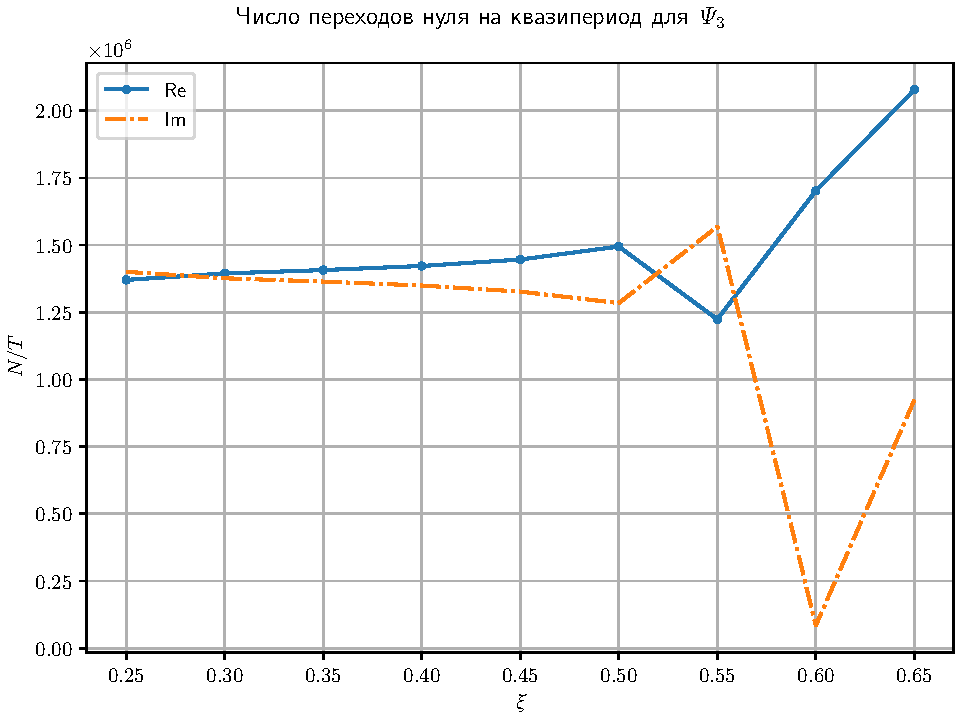
\includegraphics[width=\linewidth]{psi3-rel-trans-ru}
\end{frame}

\begin{frame}
  \frametitle{Заключение}%
  %%%
  В данной работе мы применили встроенные в Mathematica средства численного
  решения дифференциальных уравнений (DOPRI) для выясления качественных
  характеристик полученного решения. 
  \begin{itemize}
  \onslide<2->%
  \item<1-> Мы нашли подходящую характеристику.
  \onslide<3->%
  \item<2->следует внимательно относиться к расчётам с помощью встроенных средств и, по возможности, использовать альтернативные алгоритмы.
  \end{itemize}
\end{frame}

\begin{frame}
  \frametitle{КОНЕЦ}%
  \LARGE%
  \centering%
  \bfseries%
  СПАСИБО ЗА ВНИМАНИЕ%
\end{frame}

\begin{frame}
  \frametitle{Дополнительно}%
  %%%
  \centering%
  ДОПОЛНИТЕЛЬНЫЙ МАТЕРИАЛ
\end{frame}

\end{document}

%%% Local Variables:
%%% mode: latex
%%% fill-column: 80
%%% TeX-master: t
%%% TeX-PDF-mode: t
%%% End:
%%% vim: syn=tex ft=tex tw=80 ts=2 sw=2 et:


% \setbeameroption{show notes on second screen}
\setbeameroption{hide notes}
\mode<presentation>
{
  \usetheme{default}
  %\usecolortheme{default} % dove, beaver
  \usecolortheme{whale}
  %\usefonttheme{serif}
}

\hypersetup{%
  pdfinfo={%
    Title={Защита курсовых работ, ИГУ},%
    Subject={О воспроизводимости результатов численных решений уравнения осцилляции нейтрино в среде},%
    Author={Данеко Илья},%
    Keywords={neutrino oscillation in matter;quality properties}%
  }
}

\title{Качественные свойства решений уравнения осцилляций нейтрино в среде
}%
\author{Данеко И.И.}
\date[ИГУ, 2025]{%
  20 октября 2025\\%
  \vspace*{10ex}%
  \begin{flushright}
    \small
    Научный руководитель: Ломов В.П.\par
  \end{flushright}
  {\vspace*{7ex}
    \footnotesize%
    Иркутск, ФГБОУ ВО ИГУ\par%
  } }

\begin{document}

\begin{frame}
  \titlepage
\end{frame}

\begin{frame}
  \frametitle{Введение}%
  %%%
  % TODO:
  \begin{itemize}
  \item<1->
   Нейтрино — одна из самых необычных частиц в нашем мире.
   
   \item<2->
   Она обладает нулевым зарядом, полуцелым спином и участвует только в слабом
   взаимодействии.
  
  \item<3-> 
  Нейтрино существует как бы в двух видах: флейворные нейтрино и
  массивные. Первые рождаются, тогда как вторые — распространяются.
 
  
  \item<4->% 
   В данной работе мы разбираем качественные
  характеристики численного решения уравнения осцилляции нейтрино в среде.
  \end{itemize}
\end{frame}

\begin{frame}
  \frametitle{Осцилляции нейтрино}%
  %%%
  Три известных состояния флейворных  \({\nu_{\alpha}}(\alpha= e, \mu, \tau)\) являются линейными комбинациями состояний массивных \({\nu_{i}}\) c массами \(m_{i}(i=1,2,3)\), состояния флейворных нейтрино являются суперпозицией состояний массивные нейтрино
  
  \onslide<2->%
  \begin{equation*}\label{eq:1}
  	{\nu_{\alpha}}=\sum_{i}U_{\alpha i}^{*}{\nu_{i}},
  \end{equation*} 
  \(U_{\alpha i}\) являются элементами унитарной матрицы
  смешивания и называемой матрицей Понтекорва–Маки–Накагавы–Сакаты (PMNS).
  
  \onslide<3->%
  Вероятность иметь состояние аромата \(\beta\) в точке r
  \begin{equation*}
  	P_{\alpha\beta}=\sum_{j}|U_{\beta j}|^{2}|A_{j}|^{2}+2\sum_{i>j}Re[U_{\beta i}U_{\beta j}^{*}A_{i}A_{j}^{*}\exp^{-\imath\Delta_{ij}L}].
  \end{equation*}
  Здесь \(\Delta_{ij}=\Delta m_{ij}^2/2E\), где \(E=|p|\), а \(A_{i}\) амплитуда вероятности наличия в точке регестрации
\end{frame}

\begin{frame}
  \frametitle{Осцилляции нейтрино в веществе}%
  %%%
  Уравнение осцилляций в среде
  \begin{equation*}
  	\imath \frac{\partial \Psi}{\partial \xi}=H(\xi)\Psi(\xi).\quad
  \end{equation*}
   \onslide<2->%
  Здесь \({H(\xi)}\) — эрмиртовая матрица
  \begin{equation*}
  	H(\xi)=H_0+\upsilon(\xi)W
  \end{equation*}
   \onslide<3->%
  Матрица \(W\) имеет вид:
  \begin{equation*}
  	W=
  	\begin{pmatrix}
  		c_{13}^{2}c_{12}^{2} & c_{12}s_{12}c_{13}^{2} & c_{12}c_{13}s_{13}\\
  		c_{12}s_{12}c_{13}^{2} & s_{12}^{2}c_{13}^{2} & s_{12}c_{13}s_{13}\\
  		c_{12}s_{13}c_{13} & s_{12}c_{13}s_{13} & s_{13}^{2}
  	\end{pmatrix}.
  \end{equation*}

  \onslide<4->%
  Профиль плотности для солнечной модели
  
  \begin{equation*}
  	\upsilon(\xi)=\gamma exp(-\eta\xi)
  \end{equation*}
  

\end{frame}

\begin{frame}
  \frametitle{Наблюдаемые}%
  %%%
  Вероятность иметь состояние аромата \(\beta\) в точке r
  \begin{equation*}
  	P_{\alpha\beta}=\sum_{j}|U_{\beta j}|^{2}|A_{j}|^{2}+2\sum_{i>j}Re[U_{\beta i}U_{\beta j}^{*}A_{i}A_{j}^{*}\exp(-\imath\Delta_{ij}L)].
  \end{equation*}
  
  \onslide<2->%
  средняя вероятность выживания составляет
  \begin{equation}
  	\langle P_{ee} \rangle=c_{12}^{2}c_{13}^{2}|\Psi_{1}|^{2}+s_{12}^{2}c_{13}^{2}|\Psi_{2}|^{2}+s_{13}^{2}|\Psi_{3}|^{2}.
  \end{equation}
\end{frame}

\begin{frame}
	\frametitle{Качественные свойства решения}%
	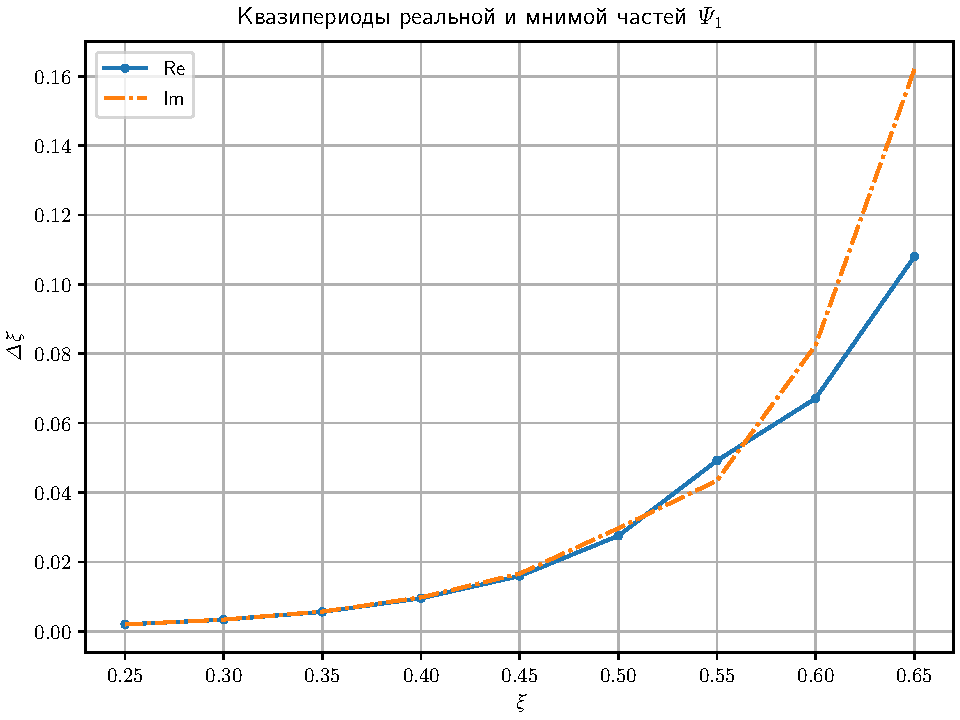
\includegraphics[width=\linewidth]{ri-widths-ru}
\end{frame}

\begin{frame}
	\frametitle{Качественные свойства решения}%
	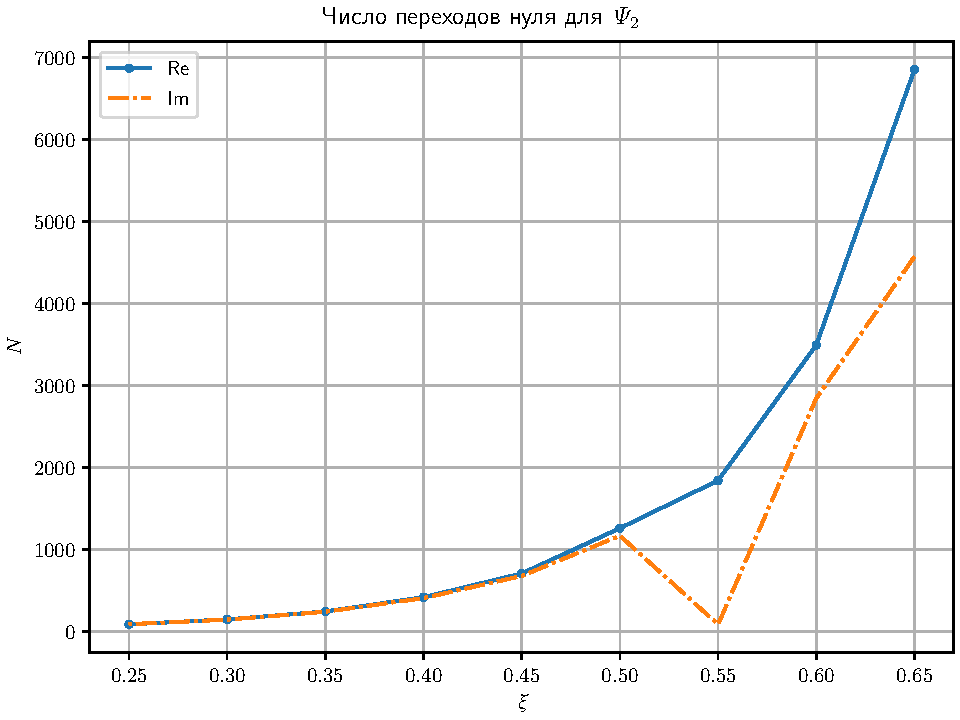
\includegraphics[width=\linewidth]{psi2-trans-ru}
\end{frame}

\begin{frame}
	\frametitle{Качественные свойства решения}%
	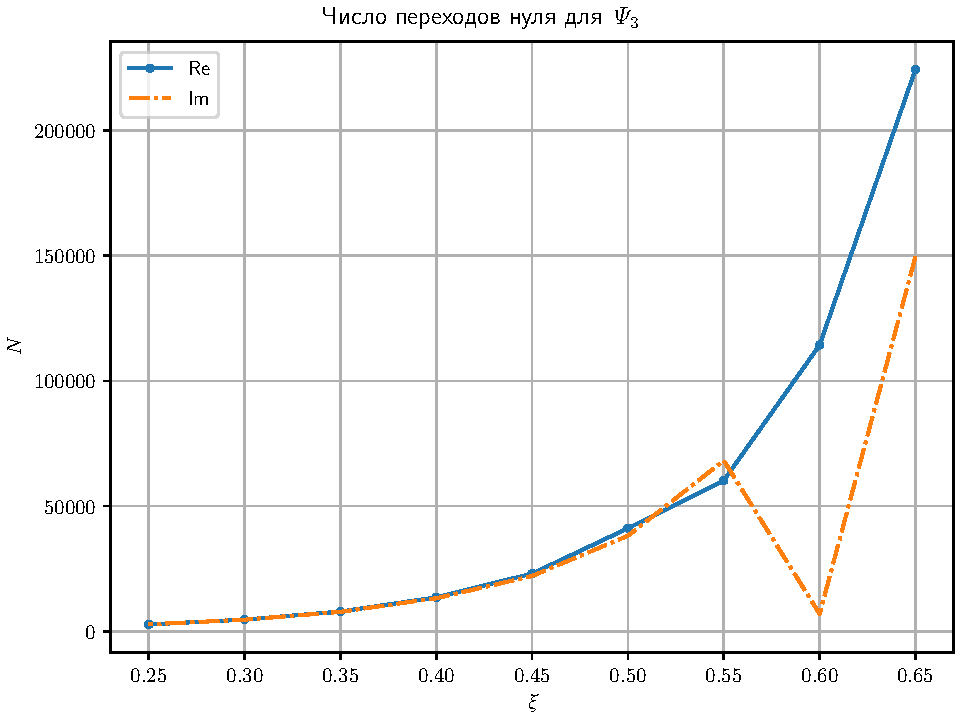
\includegraphics[width=\linewidth]{psi3-trans-ru}
\end{frame}

\begin{frame}
	\frametitle{Качественные свойства решения}%
	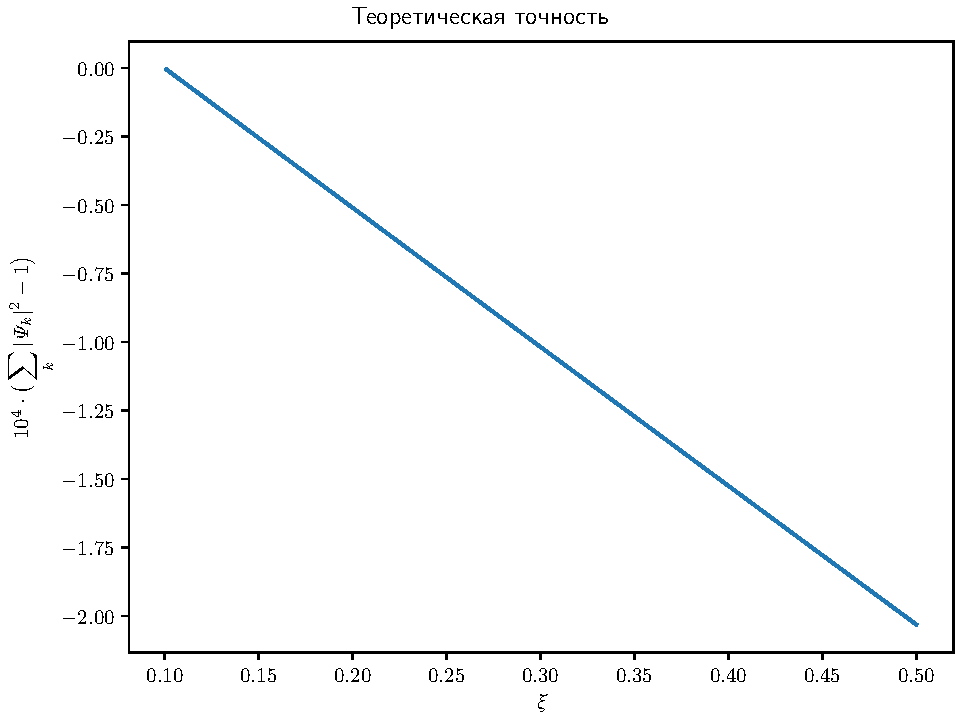
\includegraphics[width=\linewidth]{control-scaled}
\end{frame}

\begin{frame}
	\frametitle{Качественные свойства решения}%
	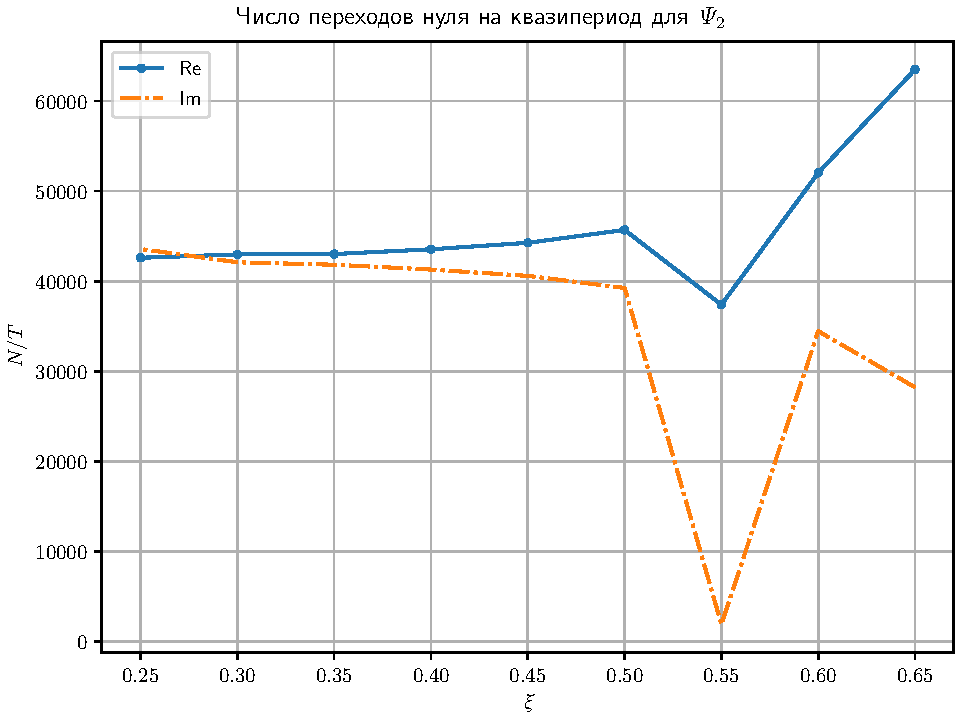
\includegraphics[width=\linewidth]{psi2-rel-trans-ru}
\end{frame}

\begin{frame}
	\frametitle{Качественные свойства решения}%
	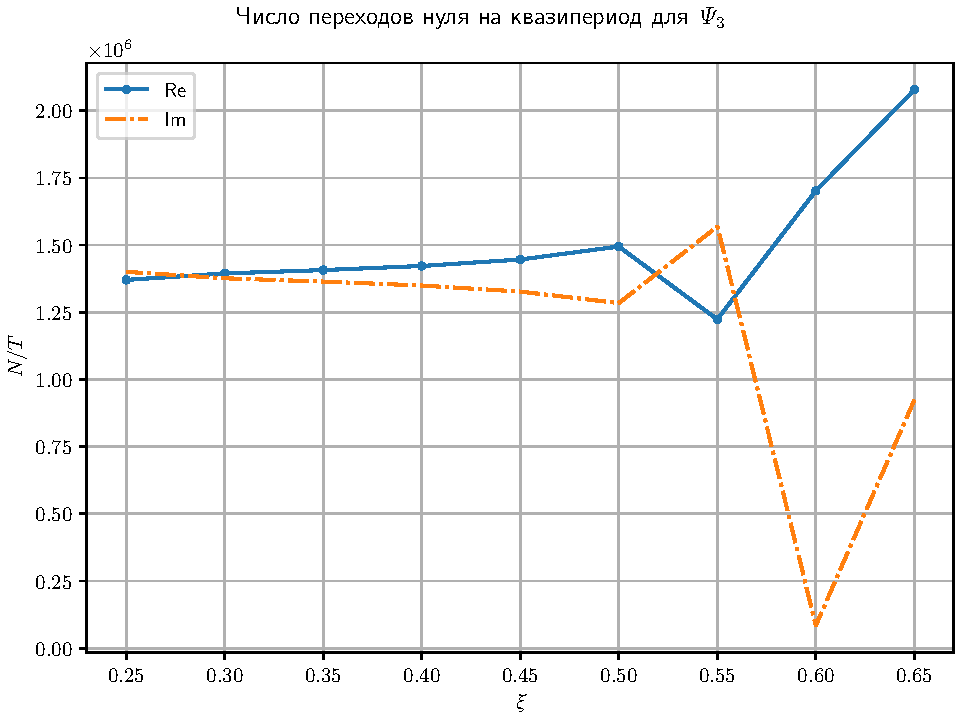
\includegraphics[width=\linewidth]{psi3-rel-trans-ru}
\end{frame}

\begin{frame}
  \frametitle{Заключение}%
  %%%
  В данной работе мы применили встроенные в Mathematica средства численного
  решения дифференциальных уравнений (DOPRI) для выясления качественных
  характеристик полученного решения. 
  \begin{itemize}
  \onslide<2->%
  \item<1-> Мы нашли подходящую характеристику.
  \onslide<3->%
  \item<2->следует внимательно относиться к расчётам с помощью встроенных средств и, по возможности, использовать альтернативные алгоритмы.
  \end{itemize}
\end{frame}

\begin{frame}
  \frametitle{КОНЕЦ}%
  \LARGE%
  \centering%
  \bfseries%
  СПАСИБО ЗА ВНИМАНИЕ%
\end{frame}

\begin{frame}
  \frametitle{Дополнительно}%
  %%%
  \centering%
  ДОПОЛНИТЕЛЬНЫЙ МАТЕРИАЛ
\end{frame}

\end{document}

%%% Local Variables:
%%% mode: latex
%%% fill-column: 80
%%% TeX-master: t
%%% TeX-PDF-mode: t
%%% End:
%%% vim: syn=tex ft=tex tw=80 ts=2 sw=2 et:


% \setbeameroption{show notes on second screen}
\setbeameroption{hide notes}
\mode<presentation>
{
  \usetheme{default}
  %\usecolortheme{default} % dove, beaver
  \usecolortheme{whale}
  %\usefonttheme{serif}
}

\hypersetup{%
  pdfinfo={%
    Title={Защита курсовых работ, ИГУ},%
    Subject={О воспроизводимости результатов численных решений уравнения осцилляции нейтрино в среде},%
    Author={Данеко Илья},%
    Keywords={neutrino oscillation in matter;quality properties}%
  }
}

\title{О воспроизводимости результатов численных решений уравнения осцилляции нейтрино в среде}%
\author{Данеко И.И.}
\date[ИГУ, 2025]{%
  20 октября 2025\\%
  \vspace*{10ex}%
  \begin{flushright}
    \small
    Научный руководитель: Ломов В.П.\par
  \end{flushright}
  {\vspace*{7ex}
    \footnotesize%
    Иркутск, ФГБОУ ВО ИГУ\par%
  } }

\begin{document}

\begin{frame}
  \titlepage
\end{frame}

\begin{frame}
  \frametitle{Введение}%
  %%%
  % TODO:
  \begin{itemize}
  \item<1-> Нейтрино...
  \item<2-> Осцилляции в среде...
  \item<3-> Проблемы численных расчётов.
  \end{itemize}
  \onslide<4->%
  В данной работе мы ...
\end{frame}

\begin{frame}
  \frametitle{Осцилляции нейтрино}%
  %%%
  Что такое нейтрино

  \onslide<2->%
  Массивные нейтрино...

  \onslide<3->%
  Переход от одного вида к другому
\end{frame}

\begin{frame}
  \frametitle{Осцилляции нейтрино в веществе}%
  %%%
  Уравнение осцилляций

  \onslide<2->%
  Профиль плотности для солнечной модели

  \onslide<3->%
  ...
\end{frame}

\begin{frame}
  \frametitle{Наблюдаемые}%
  %%%
  Вероятность выживания

  \onslide<2->
  Теоретическая формула
\end{frame}

\begin{frame}
  \frametitle{Качественные свойства решения}%
  %%%
  %\includegraphics{graph1}
  График 1
\end{frame}

\begin{frame}
  \frametitle{Качественные свойства решения}%
  %%%
  %\includegraphics{graph2}
  График 2
\end{frame}

\begin{frame}
  \frametitle{Качественные свойства решения}%
  %%%
  %\includegraphics{graph3}
  График 3
\end{frame}

\begin{frame}
  \frametitle{Качественные свойства решения}%
  %%%
  %\includegraphics{quality}
  Контроль качества решения:
  График 4
\end{frame}

\begin{frame}
  \frametitle{Заключение}%
  %%%
  В данной работы мы получили
  \begin{itemize}
  \item<1-> что-то хорошее
  \item<2-> не очень хорошее, но можно сделать в будущем (лучше?)
  \end{itemize}
\end{frame}

\begin{frame}
  \frametitle{КОНЕЦ}%
  \LARGE%
  \centering%
  \bfseries%
  СПАСИБО ЗА ВНИМАНИЕ%
\end{frame}

\begin{frame}
  \frametitle{Дополнительно}%
  %%%
  \centering%
  ДОПОЛНИТЕЛЬНЫЙ МАТЕРИАЛ
\end{frame}

\begin{frame}
  \frametitle{Введение}%
  Основной целью данной работы является исследование воспроизводимости
  результатов численных решений уравнения осцилляции нейтрино в среде. В
  соответствии с целью были поставлены следующие задачи исследования:
  \begin{itemize}
  \item<1->Ознакомиться с доступной информацией по методам, используемым в
    статье 2016 года “ Efficient numerical integration of neutrino oscillations
    in matter” (Эффективное численное интегрирование нейтринных осцилляций в
    веществе)
  \item<2-> Повторить в Mathematica вычисления, произведённые в статье.
  \item<3->Проверить насколько изменение неуказанных в статье параметров влияет
    на результат
  \end{itemize}
\end{frame}

\begin{frame}
  \frametitle{Уравнения осцилляции}%
 Уравнения осцилляции
  \begin{equation*}
    \imath \frac{\partial \Psi}{\partial \xi}=H(\xi)\Psi(\xi),\quad
  \end{equation*}
  \onslide<2->%
   Здесь \(\Vect{H(\xi)}\) — Эрмитова матрица
  \begin{equation*}
    H(\xi)=H_0+\upsilon(\xi)W
  \end{equation*}
  \onslide<3->%
  Средняя вероятность выживания
  \begin{equation*}
    P_{ee}=c_{12}^2c_{13}^2\rho_1+ s_{12}^2c_{13}^2\rho_2 + s_{13}^2\rho_3
  \end{equation*}
 Здесь \(\Vect{\rho_i(\xi)}=|\Psi_i(\xi)|^2\)
\end{frame}

\begin{frame}
  \frametitle{Ошибка Mathematica}%
\begin{figure}[h!]
\centering

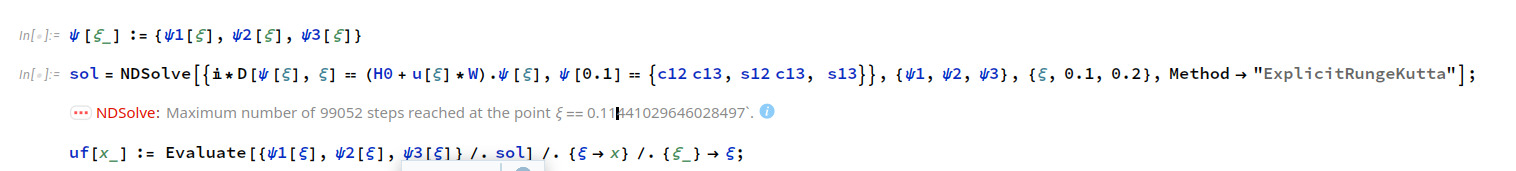
\includegraphics[width=1\linewidth]{Снимок.jpg}

\caption{1 — Ошибка возникшая при указании метода}

\label{fig:mpr}

\end{figure}
\end{frame}

\begin{frame}
  \frametitle{Погрешности}%
Уравнение для выявления погрешностей
\begin{equation*}
   \sum_{j=1}^3\rho_j=1
  \end{equation*}
\begin{figure}[h!]
\centering

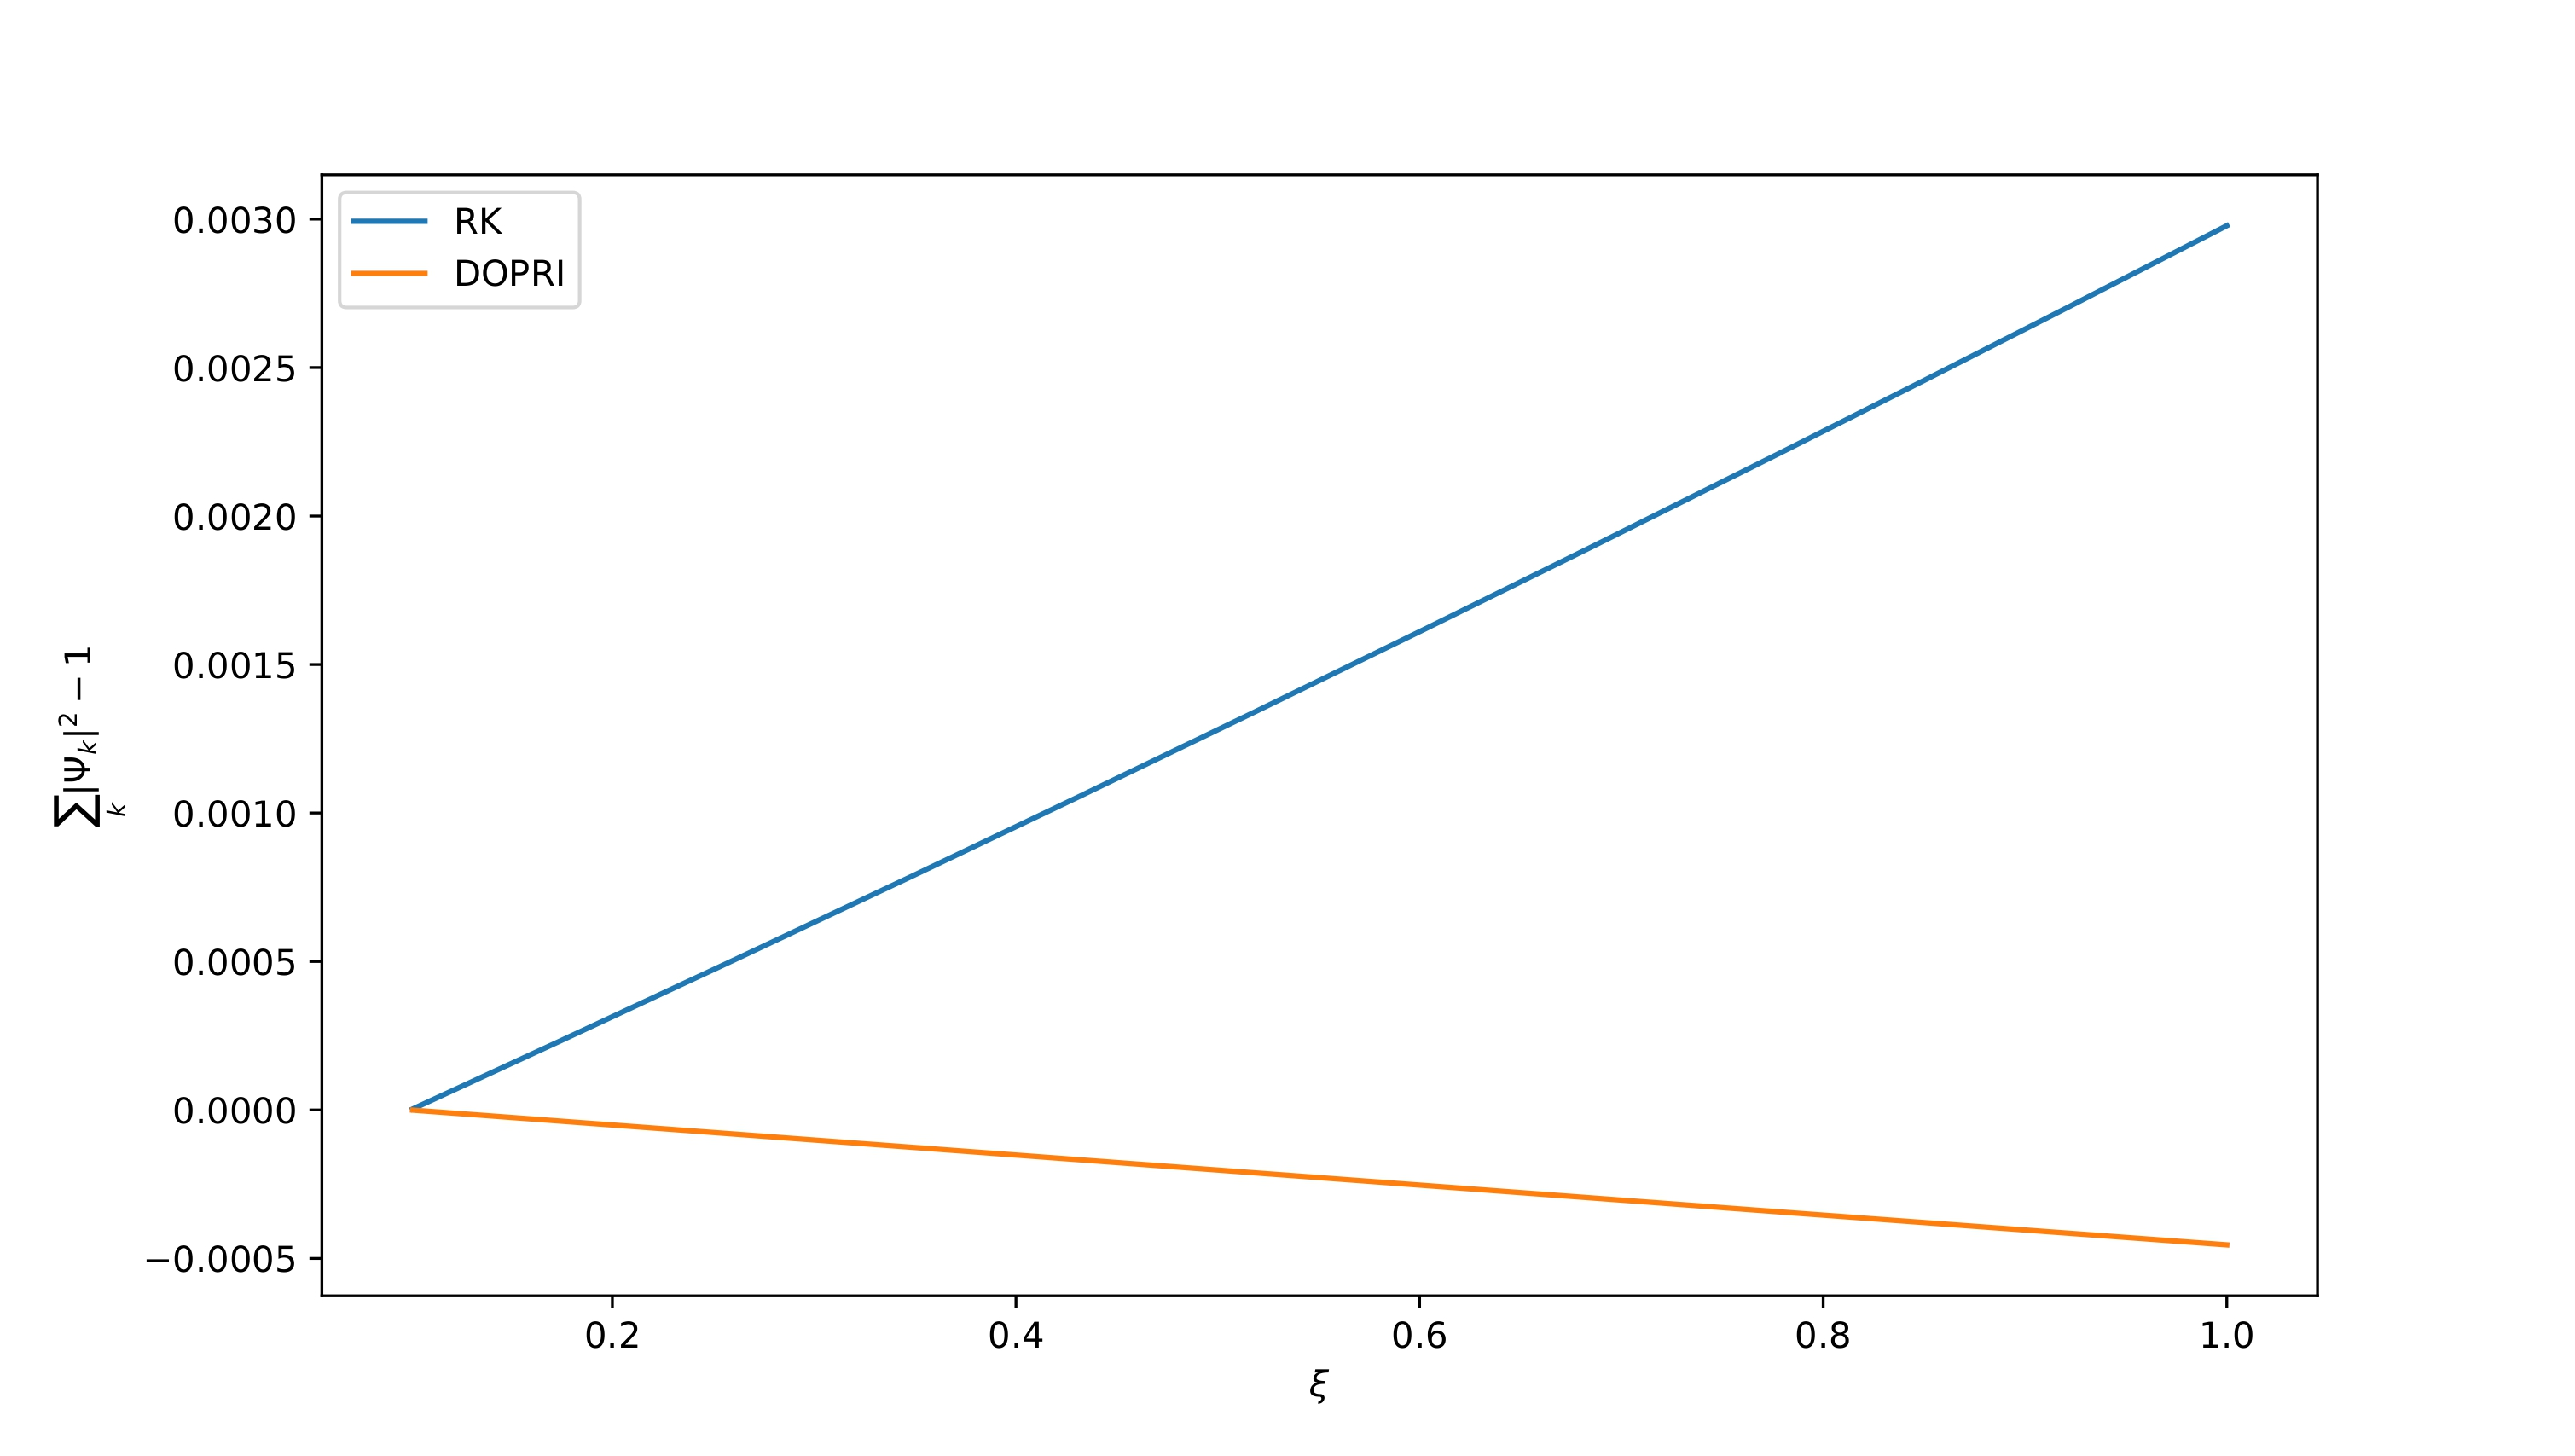
\includegraphics[width=0.8\linewidth]{1conrol_c.jpg}

\caption{2 — График погрешностей методов DOPRI и RK}

\label{fig:mpr}

\end{figure}
\end{frame}

\begin{frame}
  \frametitle{Контроль}%
\begin{figure}[h!]
\centering

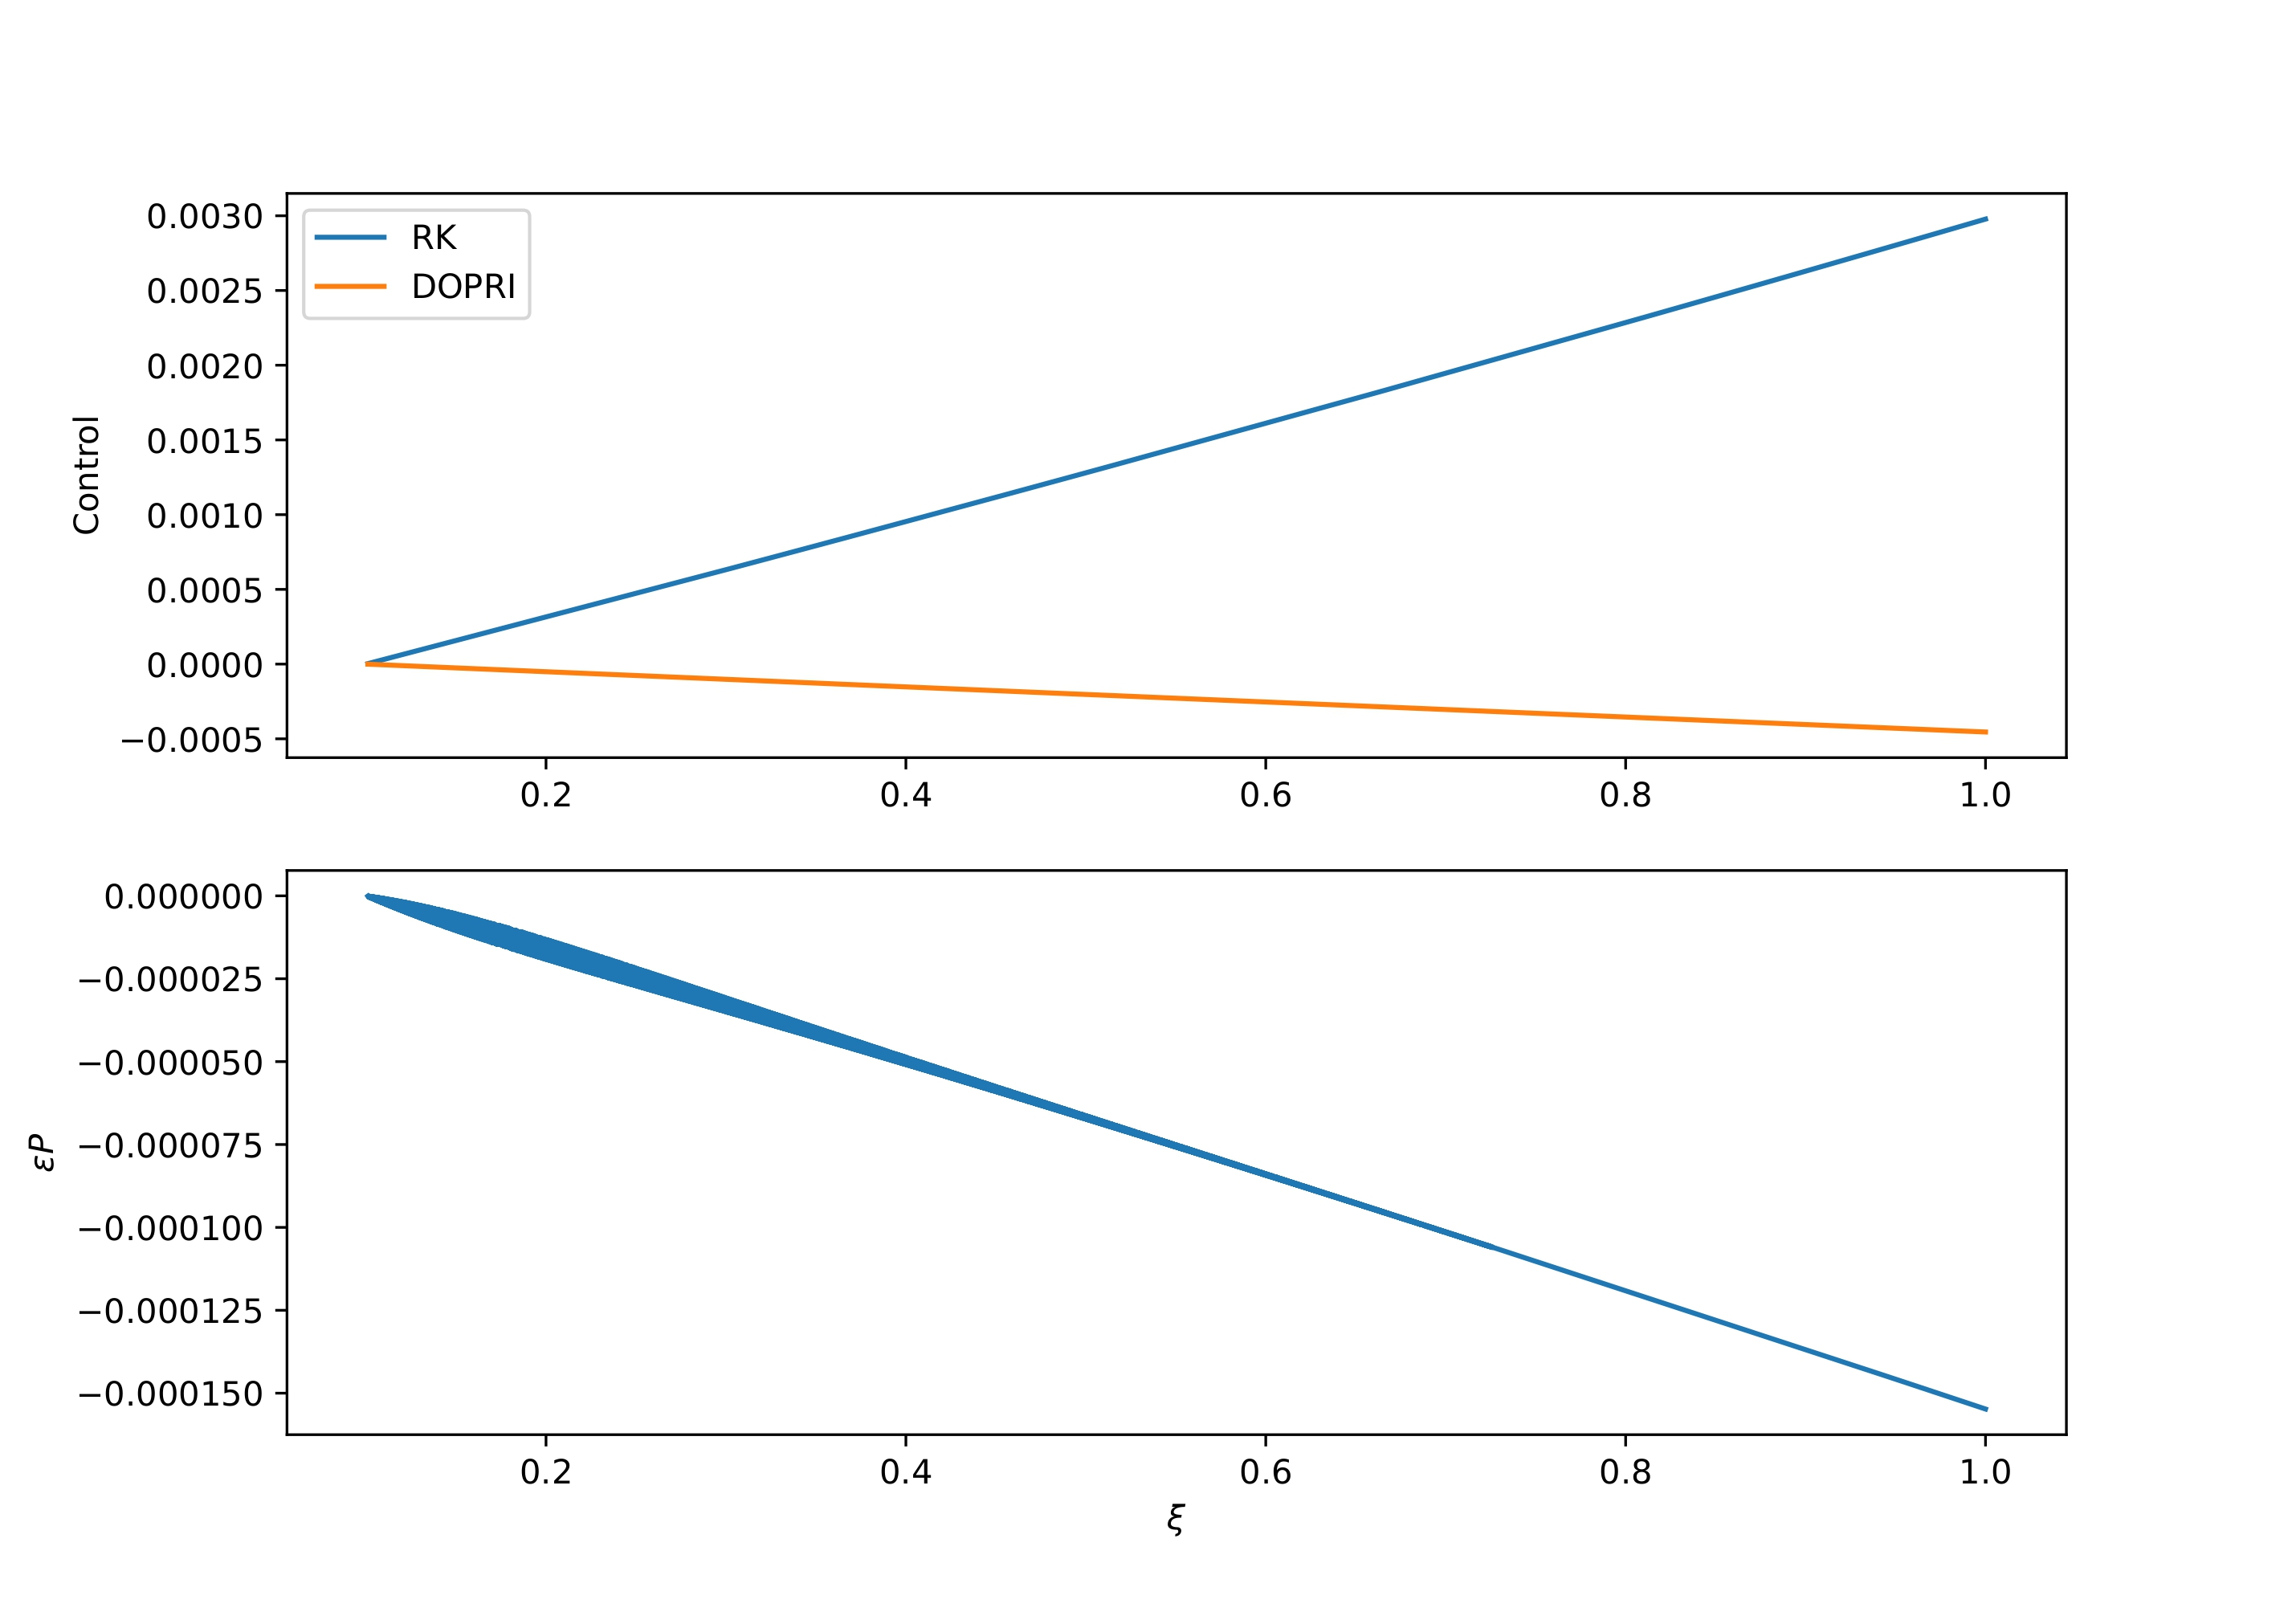
\includegraphics[width=0.8\linewidth]{(pr2-pr1)pr2.jpg}

\caption{3 — График относительной разности вероятности выживания нейтрино DOPRI и RK}

\label{fig:mpr}

\end{figure}
\end{frame}

\begin{frame}
  \frametitle{Заключение}%
  \begin{itemize}
  \item<1-> Численные расчеты без указания всех необходимых параметров невоспроизводимы, даже класса численных методов недостаточно, ведь два метода из одного класса могут давать разные результаты.
  \item<2-> Всегда необходимо проверять свойства систем дифференциальных уравнений.
  \item<3-> При использовании Mathematica задавать все возможные параметры, ведь незаданные параметры зачастую становятся неизвестными
  \end{itemize}
\end{frame}

\end{document}

%%% Local Variables:
%%% mode: latex
%%% fill-column: 80
%%% TeX-master: t
%%% TeX-PDF-mode: t
%%% End:
%%% vim: syn=tex ft=tex tw=80 ts=2 sw=2 et:
